\documentclass{bredelebeamer}

% \usepackage[english]{babel}
\usepackage{smartdiagram}
\usepackage{ragged2e}
\usepackage{chronosys}
\usepackage{tikz}
\usetikzlibrary{spy}
\usepackage{rotating}
\usepackage[absolute,overlay]{textpos}
\usepackage{tikz}
\definecolor{links}{HTML}{2A1B81}
\hypersetup{colorlinks,linkcolor=,urlcolor=links}

\usepackage{movie15}

% \usepackage{hyperref}
%             linkcolor  = blue,
%             urlcolor   = blue,
%             citecolor  = blue,
%             anchorcolor = blue

% [colorlinks = true,
%             linkcolor  = blue,
%             urlcolor   = blue,
%             citecolor  = blue,
%             anchorcolor = blue]

\usetikzlibrary{positioning,shapes.arrows}

\definecolor{myblue}{rgb}{0.29,0.5,0.74}
\definecolor{myred}{rgb}{0.73,0.32,0.3}
\definecolor{mygreen}{rgb}{0.59,0.73,0.34}
\definecolor{myviolet}{rgb}{0.49,0.39,0.62}
\definecolor{myturquoise}{rgb}{0.28,0.67,0.76}
\definecolor{myorange}{rgb}{0.97,0.58,0.27}

\usepackage{pgfplots}

\newcommand\tikzmark[1]{
  \tikz[remember picture,overlay] \coordinate (#1);
}

\usetikzlibrary{calc, positioning, shapes.arrows}
\usesmartdiagramlibrary{additions}
\usetikzlibrary{shapes.geometric}

%%%%%%%%%%%%%%%%%%%%%%%%%%%%%%%%%%%%%%%%%%%%%%%%

\title[Open Data Cubes]{Open Data Cubes \tiny{ and related technology }}
% Titre du diaporama

\subtitle{upcoming data revolution for sustainable development}
% Sous-titre optionnel

\author{Nils Hempelmann\inst{1,2} et. al\inst{2} }
% La commande \inst{...} Permet d'afficher l' affiliation de l'intervenant.
% Si il y a plusieurs intervenants: Marcel Dupont\inst{1}, Roger Durand\inst{2}
% Il suffit alors d'ajouter un autre institut sur le modèle ci-dessous.

\institute[ GIZ - Cameroon ]
{
  \inst{1} GIZ - Regional Project Central Africa, COMIFAC\\
  \inst{2} FOSS4G Community (OpenDataCubes, birdhouse, PAVICS, etc...)\\
}

\date{21. Juni 2018}
% Optionnel. La date, généralement celle du jour de la conférence

\subject{Sujet de votre diaporama}
% C'est utilisé dans les métadonnes du PDF

\logo{
\includegraphics[scale=0.05]{images/birdhouse.png}
}

%%%%%%%%%%%%%%%%%%%%%%%%%%%%%%%%%%%%%%%%%%%%%%%%%%%%%%%%%%%%%%%%%%%%%

\begin{document}

\begin{frame}
  \titlepage
\end{frame}

\begin{frame}{Content}
  \tableofcontents
  % possibilité d'ajouter l'option [pausesections]
\end{frame}


\section[Intro]{ Introduction }
\AtBeginSection[]
{
  \begin{frame}<beamer>
    \frametitle{Examples \thesection}
    \tableofcontents[currentsection]
  \end{frame}
}
\begin{frame}

\frametitle{Need of action}
    \centering
       \begin{tikzpicture} %[spy using overlays]
        \node (pic1) [inner sep=-30pt] {\includegraphics[height=0.588\textheight]{images/SDGs.png}};
% \only<2>{\spy[overlay,width=7cm,height=2cm,magnification=2] on (0,0) in node[] at (2,-3);}
\node [anchor=west, xshift=1.0cm, align=left] at (pic1.south east) {Sustainable \\ Development \\  Goals (SDGs)};

\node (pic2) [inner sep=0pt, anchor=south, yshift=.4cm, xshift=1.5cm, rotate=-20] at (pic1.east) {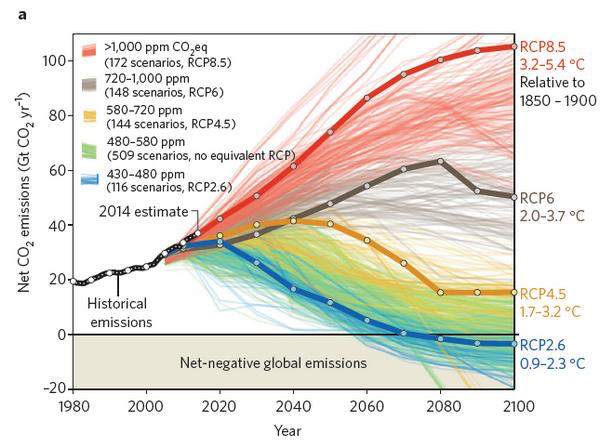
\includegraphics[width=0.3\textwidth]{images/rcps.jpg}}; %
\node [anchor=south, yshift=-.5pt, rotate=-20, align=left] at (pic2.north) {Representative\\ Carbon\\Pathways (RCPs)};

\node (pic3) [inner sep=0pt, anchor=south, xshift=-40pt, rotate=15] at (pic1.north west) {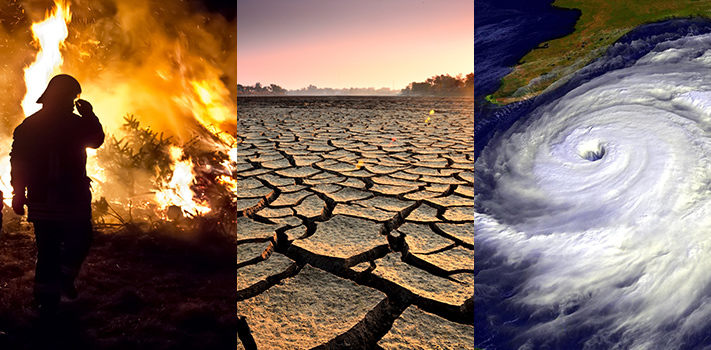
\includegraphics[width=0.5\textwidth]{images/1320_effects-image.jpg}};
\node [anchor=south, rotate=15] at (pic3.north) {\href{https://climate.nasa.gov/effects/}{nasa.gov/effects}};

\node (pic4) [inner sep=0pt, anchor=east, rotate=-5] at (pic1.south west) {\includegraphics[width=0.5\textwidth]{images/Yaounde-flooding.jpg}};
\node [anchor=south, rotate=-5] at (pic4.north) {\href{http://www.cameroonintelligencereport.com/french-cameroun-hundreds-evacuated-as-flooding-hits-yaounde/}{Cameroon Flood at 27.02.2018}};

       \end{tikzpicture}
\end{frame}


\begin{frame}

\frametitle{Growing amount of available data}

\begin{center}
 \includegraphics[width=\textwidth,keepaspectratio=true]{./images/gbif-data-portal-ecpgr-working-group-20170316-5-1024.jpg}
 % gbif-data-portal-ecpgr-working-group-20170316-5-1024.jpg: 0x0 pixel, 300dpi, 0.00x0.00 cm, bb=
\end{center}
\href{https://www.gbif.org/}{Global Biodiversity Facillity}

\end{frame}



\begin{frame}

\frametitle{Predicted EO-data availability for Australia}

\begin{center}
 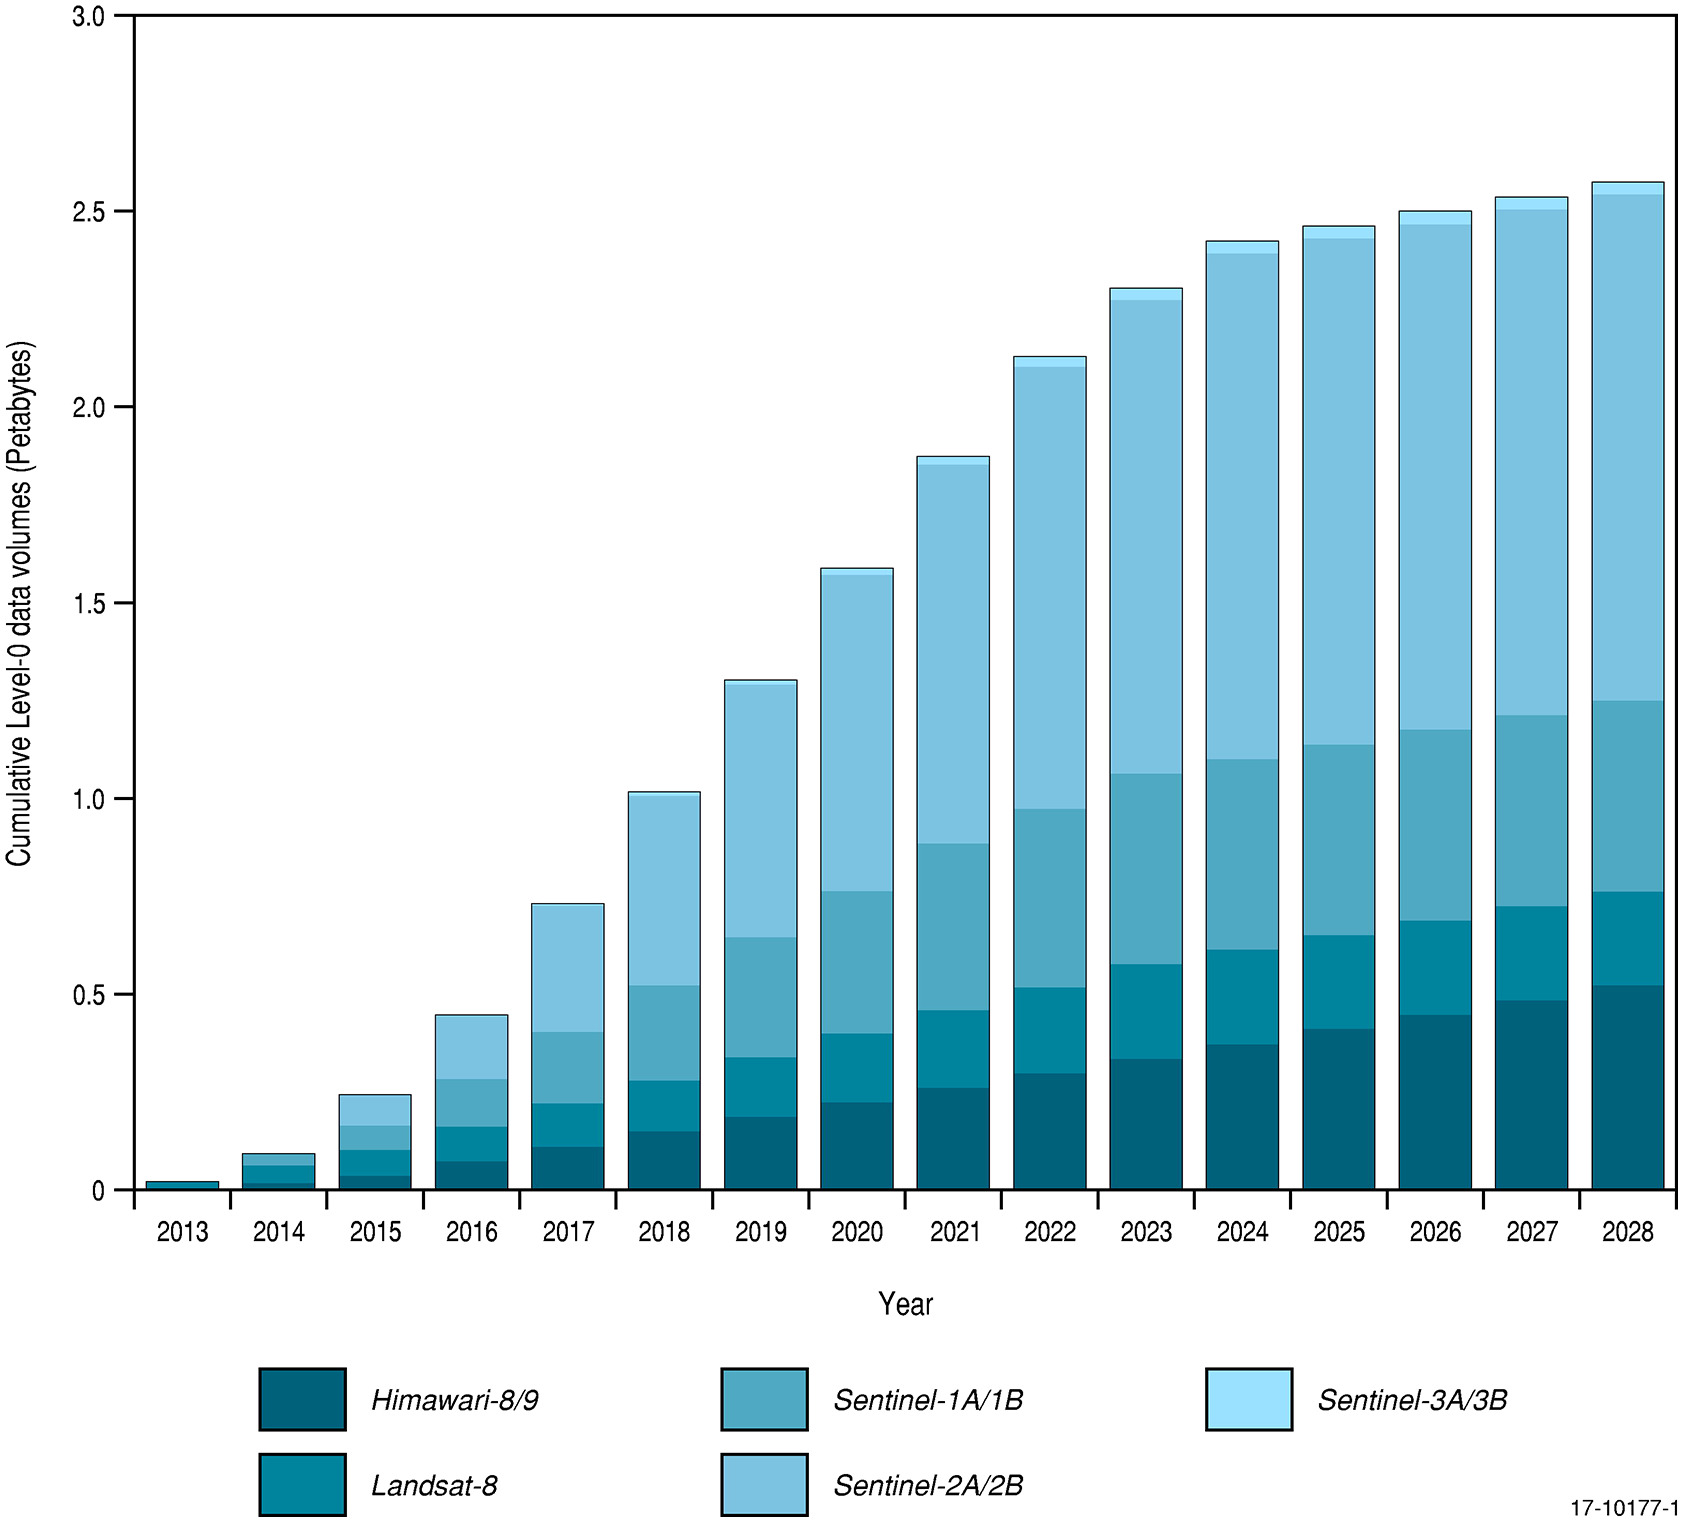
\includegraphics[height=0.8\textheight]{./images/eo-dataamount_australia.jpg}
 % earth-on-aws-nextgeneration-open-data-platforms-24-1024.jpg: 0x0 pixel, 300dpi, 0.00x0.00 cm, bb=
\end{center}

\href{http://nci.org.au/services/virtual-laboratories/australian-geoscience-data-cube/}{Australian Geoscience Data Cube}

\end{frame}

\begin{frame}

\frametitle{Global Climate Model Data Availability}

\begin{columns}[T] % align columns
\begin{column}{.4\textwidth}
	\vspace{1cm}
  \begin{tikzpicture}[scale=0.8]
	\begin{axis}[
	  symbolic x coords={CMIP 1,CMIP 2,CMIP 3,CMIP 4,CMIP 5,CMIP 6},
	  xtick=data,
      ylabel={Peta-Byte},
      ylabel near ticks,
	  ]
 	  \addplot[ybar,fill=blue] coordinates {
	  (CMIP 1,  0.0000001)
 	  (CMIP 2,  0.00005)
 	  (CMIP 3,  0.035)
 	  (CMIP 4,  )
 	  (CMIP 5,  3)
 	  (CMIP 6,  15)
 	  };
	\end{axis}
  \end{tikzpicture}
\end{column}%
\hfill%
\begin{column}{.38\textwidth}
\textbf{CMIP 1:}  ~1 GB\\ % Idealized simulations of present-day climate 
\textbf{CMIP 2:} ~500 GB\\ % Idealized simulations of future climate changes
\textbf{CMIP 3:} ~35 TB\\%  : CMIP3/CMIP2 = 70) More realistic simulations (2004 – present) 
\textbf{CMIP 4:} Not existing\\
\textbf{CMIP 5:} ~3.5 PB (multi-model archive)\\ % ( including replicas, CMIP5/CMIP3 = 100)\\
\textbf{CMIP 6:} currently 10-20 PB as "ESGF" Data (real existing 10time more) \\

************************************\\
IPCC 1 : 1990\\
IPCC 2 : 1995\\
IPCC 3 : 2001\\
IPCC 4 : 2007\\
IPCC 5 : 2014\\
IPCC 6 : --> $\sim$ 2019\\
**************************\\
Global Land Outlook: 2017 \\
(Report UNCCD)
\end{column}%
\end{columns}
% % 
\vspace{0.5cm}
\href{https://cmip.llnl.gov/}{CMIP = Coupled Model Inter-comparison Project}\\
\href{http://www.ipcc.ch/}{IPCC = Intergovernmental Panel of Climate Change}

\end{frame}

\begin{frame}

\frametitle{ Global internet speed (access to information)  }

\begin{center}
 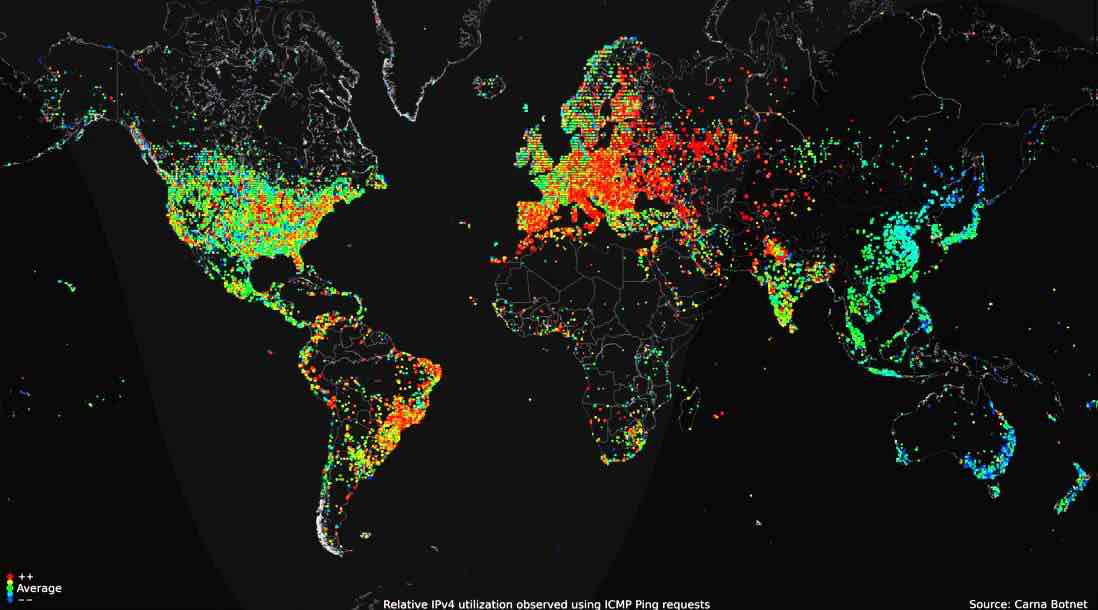
\includegraphics[width=\textwidth,keepaspectratio=true]{./images/internet-users-map-1.jpg}
 % internet-users-map-1.jpg: 0x0 pixel, 300dpi, 0.00x0.00 cm, bb=
\end{center}
\href{https://fossbytes.com/top-10-countries-having-the-fastest-average-internet-speed/}{Global Internet Speed (fossbytes.com)}

\end{frame}

\begin{frame}

\frametitle{The Big Data Problem - Download and Process at home }

\begin{tikzpicture}[
  remember picture,
  overlay,
  expl/.style={draw=orange,fill=orange!30,rounded corners,text width=0.6cm},
  arrow/.style={orange!30,ultra thick,->,>=latex}
]

\node[anchor=south west,inner sep=0]
  (worldmap)
  at (-1,-4.2)
  {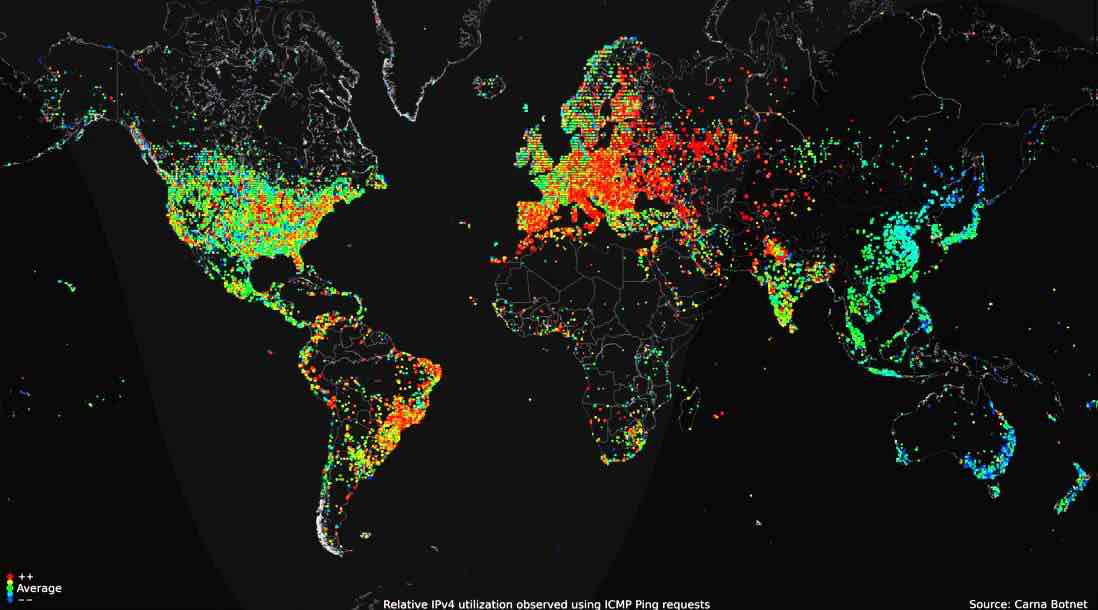
\includegraphics[width=1.2\textwidth]{./images/internet-users-map-1.jpg}}
  ;

\node[expl] 
  (data-NA) 
  at (1,0cm)
  {
\includegraphics[height=0.6cm,keepaspectratio=true]{./images/disc.png}} % 
  ;
\node[expl] 
  (data-CA) 
  at (2.5,1.5cm)
  {
\includegraphics[height=0.6cm,keepaspectratio=true]{./images/disc.png}};
\node[expl] 
  (data-AU) 
  at (10.3,-2.8cm)
  {
\includegraphics[height=0.6cm,keepaspectratio=true]{./images/disc.png}};
\node[expl] 
  (data-EU) 
  at (6.5,2cm)
  {
\includegraphics[height=0.6cm,keepaspectratio=true]{./images/disc.png}};

\node[expl] 
  (user) 
  at (5,0.5cm)
  {
\includegraphics[height=0.6cm,keepaspectratio=true]{./images/user.png}};
  
\draw[arrow]
  (data-NA.south) to[out=270,in=180] ({user}); % [yshift=0.5ex] 
\draw[arrow]
  (data-CA.west) to[out=180,in=180] ({user});  
\draw[arrow]
  (data-AU.north) to[out=90,in=0] ({user});  
\draw[arrow]
  (data-EU.west) to[out=180,in=0] ({user});  
\end{tikzpicture}
% \end{exampleblock}
\end{frame}


\begin{frame}

\frametitle{The Big Data Problem - Process in federated Networks}

\begin{tikzpicture}[
  remember picture,
  overlay,
  expl/.style={draw=orange,fill=orange!30,rounded corners,text width=0.6cm},
 % arrow/.style={red!80!black,ultra thick,->,>=latex}
  line/.style={blue!80!black,ultra thick,-,>=latex}
  arrow/.style={green!80!black,ultra thick,->,>=latex}
]

\node[anchor=south west,inner sep=0]
  (worldmap)
  at (-1,-4.2)
  {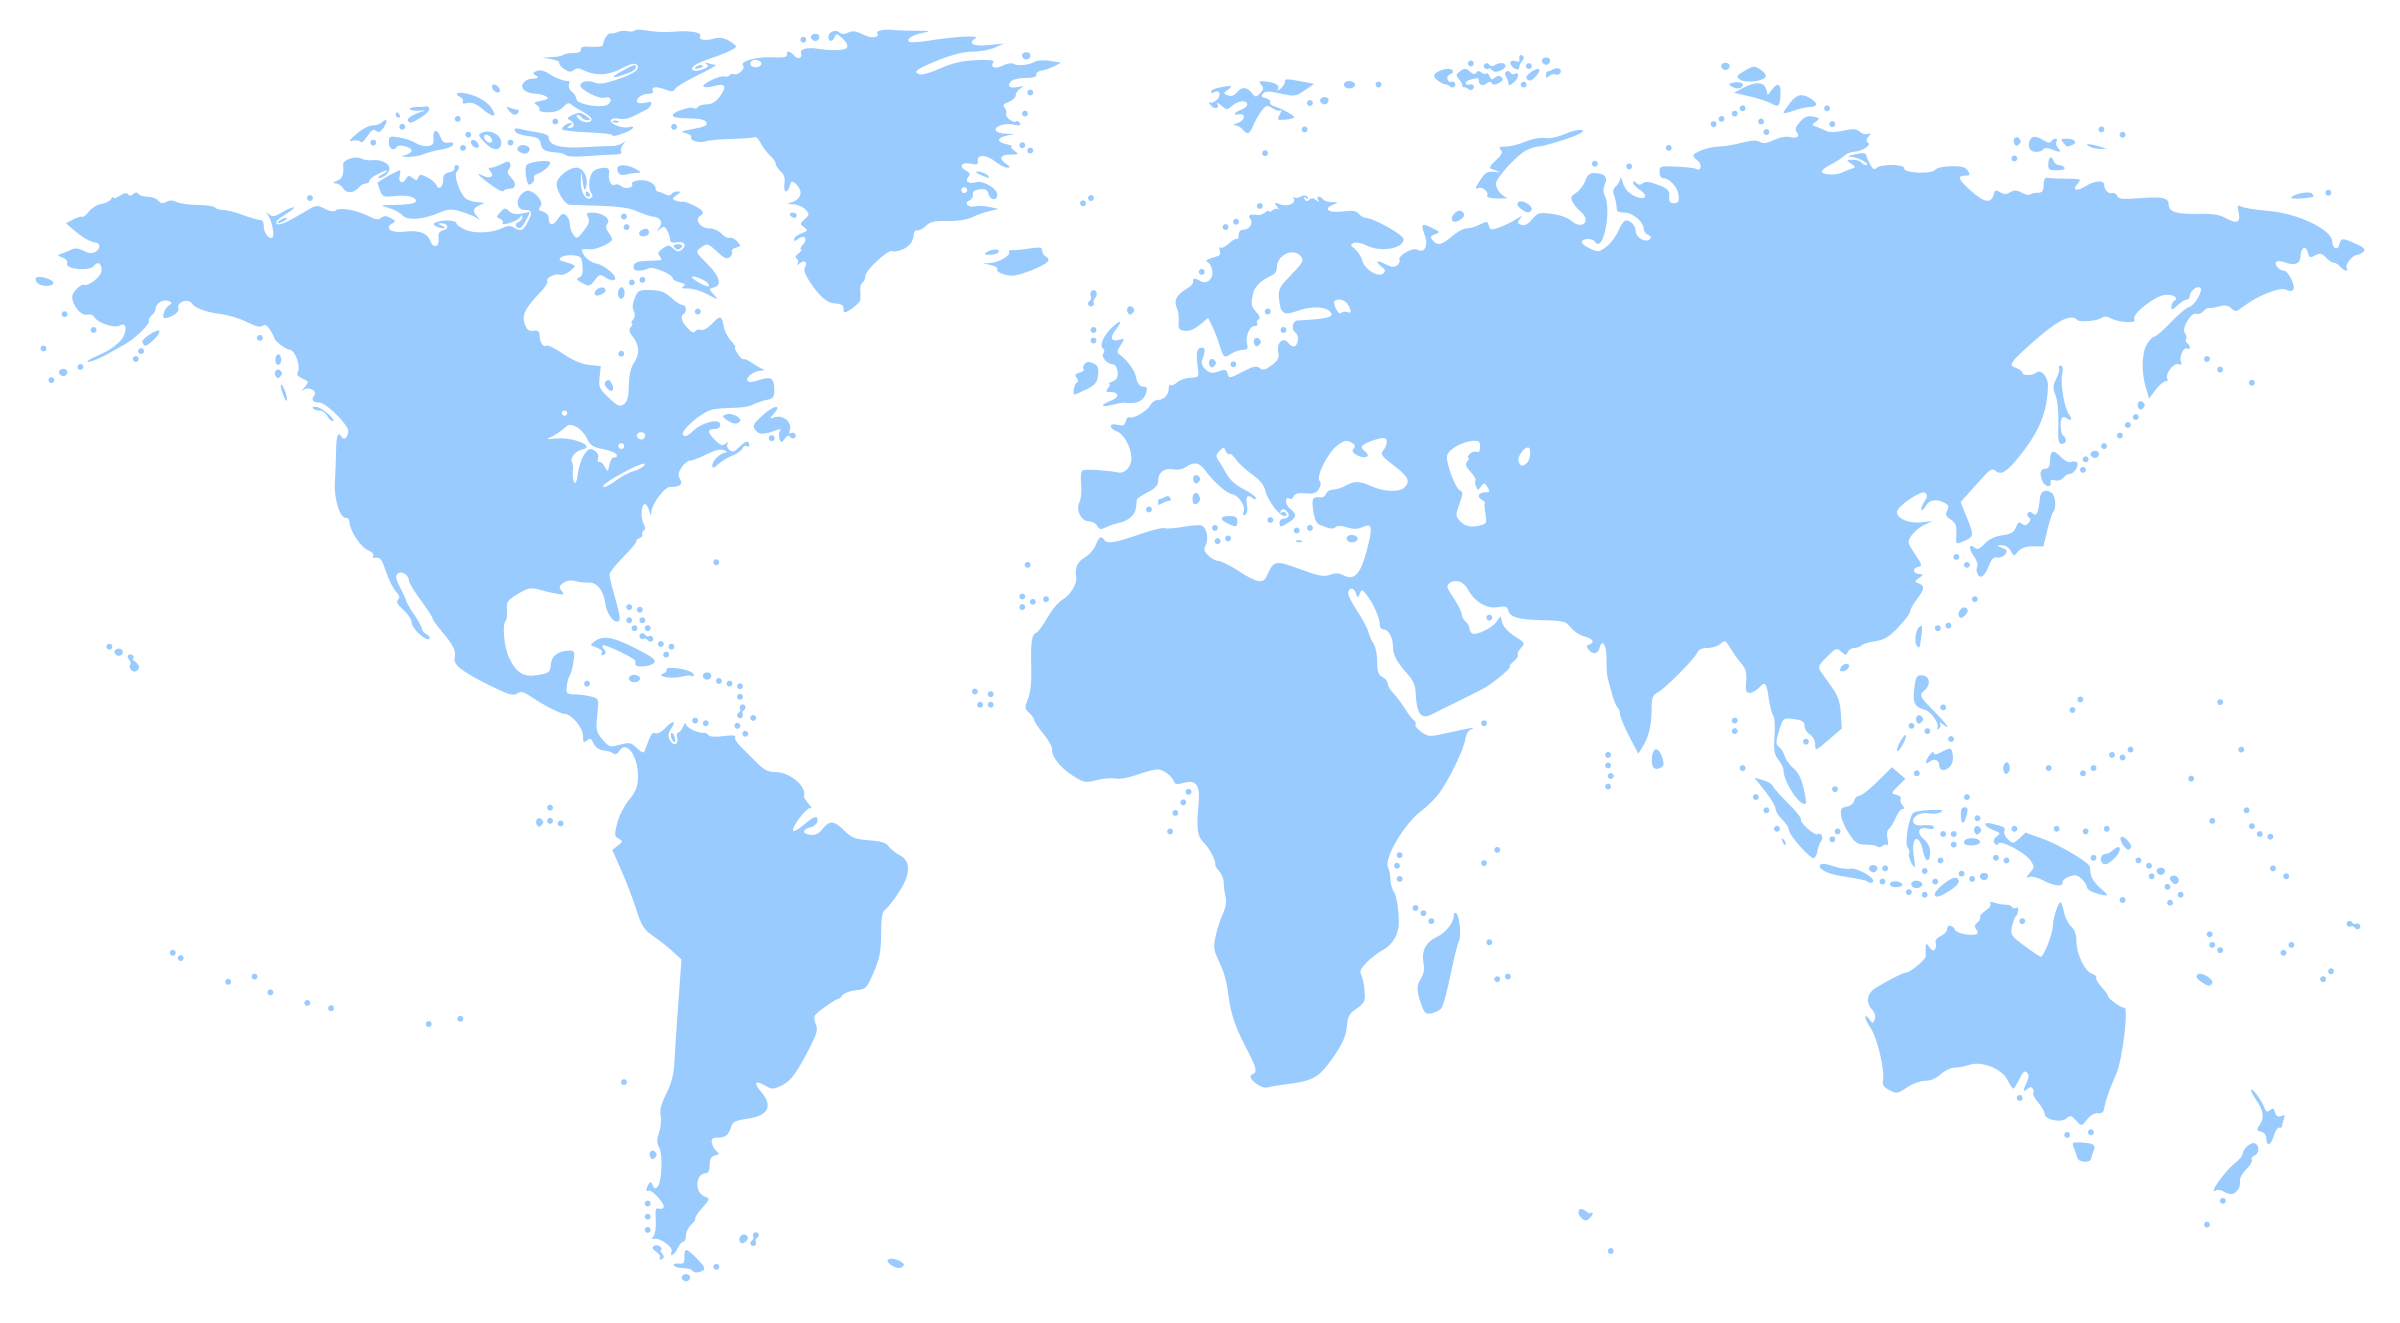
\includegraphics[width=1.2\textwidth]{./images/worldmap}}
  ;
\node[expl] 
  (data-NA) 
  at (1,0cm)
  {
\includegraphics[height=0.6cm,keepaspectratio=true]{./images/disc.png}} % 
  ;
\node[expl] 
  (data-CA) 
  at (2.5,1.5cm)
  {
\includegraphics[height=0.6cm,keepaspectratio=true]{./images/disc.png}};
\node[expl] 
  (data-AU) 
  at (9.5,-3cm)
  {
\includegraphics[height=0.6cm,keepaspectratio=true]{./images/disc.png}};
\node[expl] 
  (data-EU) 
  at (6.5,2cm)
  {
\includegraphics[height=0.6cm,keepaspectratio=true]{./images/disc.png}};

\node[expl] 
  (user) 
  at (5,0.5cm)
  {
\includegraphics[height=0.6cm,keepaspectratio=true]{./images/user.png}};
  
\draw[line]
  (data-NA.north) to[out=90,in=180] ({data-CA});  
\draw[line]
  (data-NA.south) to[out=270,in=180] ({data-AU});  
\draw[line]
  (data-NA.east) to[out=0,in=180] ({data-EU});  
  
\draw[line]
  (data-CA.south) to[out=270,in=180] ({data-AU});  
\draw[line]
  (data-CA.east) to[out=0,in=180] ({data-EU});  

\draw[line]
  (data-AU.north) to[out=90,in=0] ({data-EU});
  
\draw[line]
  (user.east) to[out=0,in=270] ({data-EU});   
\end{tikzpicture}

% \end{exampleblock}

\end{frame}

\begin{frame}

\frametitle{Big opportunity less/least developed countries }

\begin{tikzpicture}[
  remember picture,
  overlay,
  expl/.style={draw=orange,fill=orange!30,rounded corners,text width=0.6cm},
 % arrow/.style={red!80!black,ultra thick,->,>=latex}
  line/.style={blue!80!black,ultra thick,-,>=latex}
  arrow/.style={green!80!black,ultra thick,->,>=latex}
]

\node[anchor=south west,inner sep=0]
  (worldmap)
  at (-1,-4.2)
  {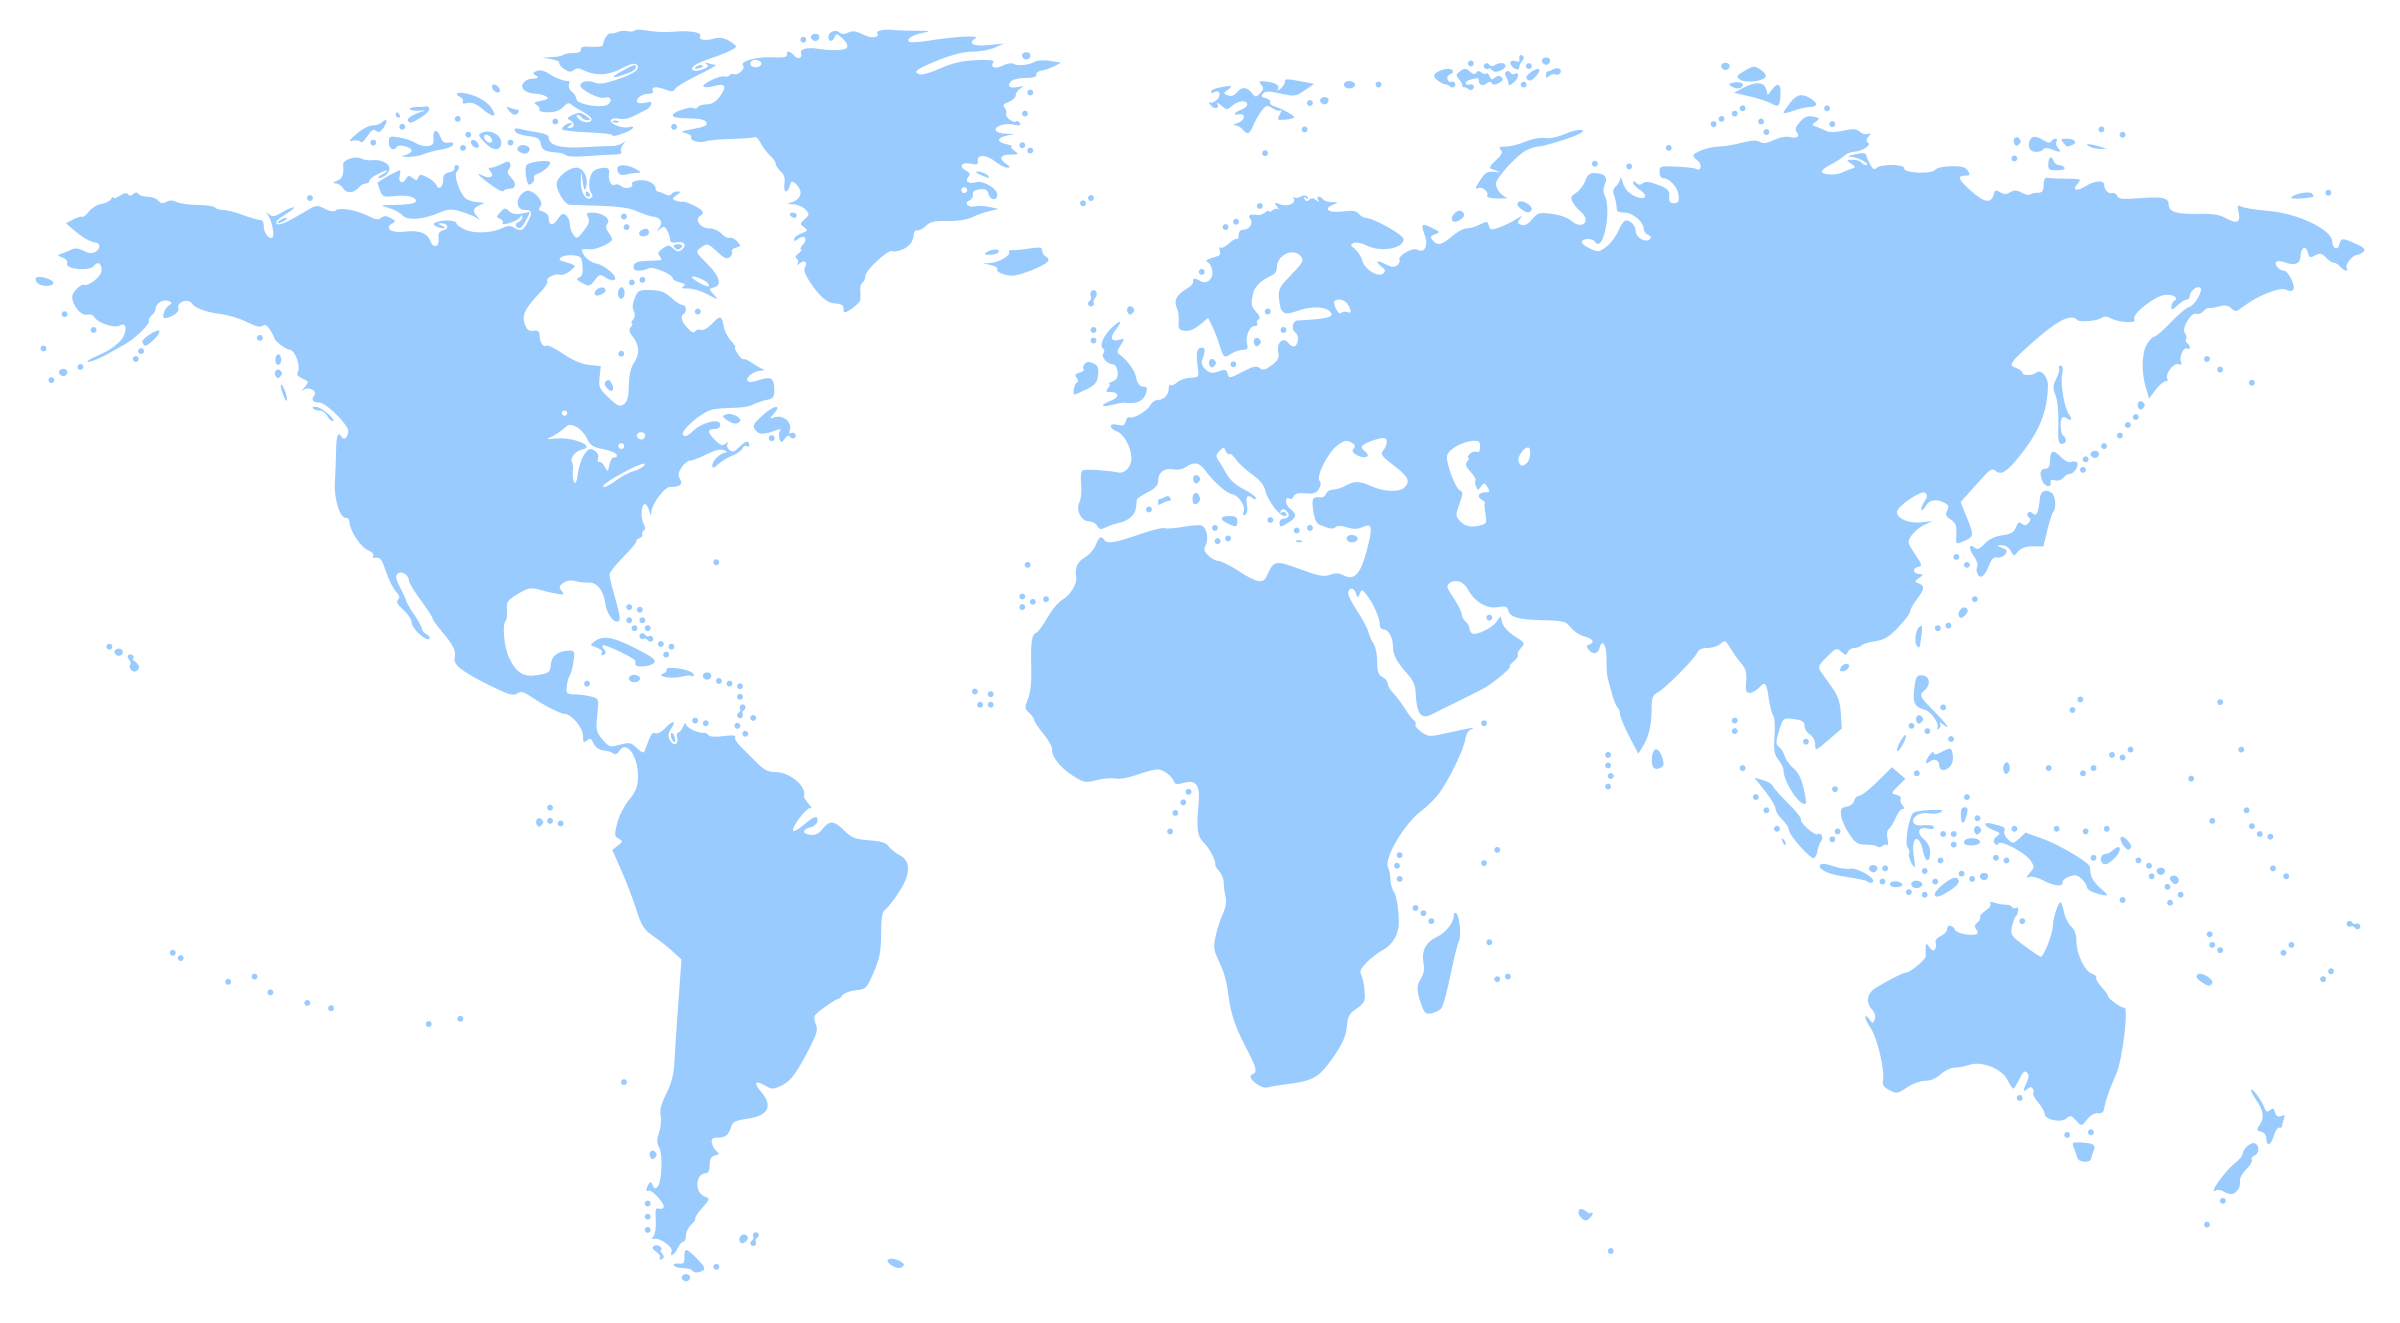
\includegraphics[width=1.2\textwidth]{./images/worldmap}}
  ;
\node[expl] 
  (data-NA) 
  at (1,0cm)
  {
\includegraphics[height=0.6cm,keepaspectratio=true]{./images/disc.png}} % 
  ;
\node[expl] 
  (data-CA) 
  at (2.5,1.5cm)
  {
\includegraphics[height=0.6cm,keepaspectratio=true]{./images/disc.png}};
\node[expl] 
  (data-AU) 
  at (9.5,-3cm)
  {
\includegraphics[height=0.6cm,keepaspectratio=true]{./images/disc.png}};
\node[expl] 
  (data-EU) 
  at (6.5,2cm)
  {
\includegraphics[height=0.6cm,keepaspectratio=true]{./images/disc.png}};

\node[expl] 
  (user) 
  at (5,0.5cm)
  {
\includegraphics[height=0.6cm,keepaspectratio=true]{./images/user.png}};

\node[expl] 
  (user2) 
  at (5.5,-1.5cm)
  {
\includegraphics[height=0.6cm,keepaspectratio=true]{./images/user.png}};
  
\draw[line]
  (data-NA.north) to[out=90,in=180] ({data-CA});  
\draw[line]
  (data-NA.south) to[out=270,in=180] ({data-AU});  
\draw[line]
  (data-NA.east) to[out=0,in=180] ({data-EU});  
  
\draw[line]
  (data-CA.south) to[out=270,in=180] ({data-AU});  
\draw[line]
  (data-CA.east) to[out=0,in=180] ({data-EU});  

\draw[line]
  (data-AU.north) to[out=90,in=0] ({data-EU});
  
\draw[line]
  (user.east) to[out=0,in=270] ({data-EU});   

\draw[line]
  (user2.east) to[out=0,in=270] ({data-EU});   

\end{tikzpicture}


% \end{exampleblock}
\end{frame}



\begin{frame}

\frametitle{Political discourse}  
\definecolor{blue}{HTML}{84CECC}
\definecolor{gr}{HTML}{375D81}


% \begin{tikzpicture}[node distance=0pt,
% 		    SA/.style = {single arrow, draw=blue!40!gray, very thick, fill=blue!20!gray!10,minimum height=1.6*\n1,}]
% \node (n) [text width=0.8\textwidth]
% \path   let \p1 = ($(n.north)-(n.south)$),
%             \n1 = {veclen(\y1,\x1)} in
%         node[SA, rotate=0,  xshift=\n1/2, above=of n.south west] {UNFCCC}
%         node[SA, rotate=0,  xshift=-\n1/2, above=of n.south east] {UNCCD};
% \end{tikzpicture}

%---------------------timeline----------------%

\startchronology[startyear=1990, stopyear=2030, arrow=true]
\chronograduation[periode]{5}

\definechronoevent{UNgen}[textstyle=\bf\raggedright\scriptsize, year=false, align=center, xshift=3cm] 

\definechronoevent{UNFCCC}[textstyle=\bf\scriptsize\raggedright\colorbox{orange!50}, barre=true,  year=false]
\definechronoevent{UNCCD}[textstyle=\bf\scriptsize\raggedright\colorbox{yellow!50}, barre=true, year=false, textwidth=2cm] 
\definechronoevent{UNCBD}[textstyle=\bf\scriptsize\colorbox{green!50}, barre=true, year=false]

% \definechronoevent{UNCBD}[textstyle=\bf, markdepth=110pt, barre=true, colorbox=green, year=true, textwidth=2cm] 
 
\chronoUNFCCC[markdepth=35pt]{1992}{UNFCCC Climate Change}
\chronoUNFCCC[markdepth=21pt]{1995}{Kyoto Protocol} %Emission reduction $5,2 \%$ until 2008-12 
\chronoUNFCCC[markdepth=9pt]{1997}{Copenhagen Agreement} %  Climate Change limit to 2
\chronoUNFCCC[markdepth=21pt]{2011}{Doha Agreement} % second Phase of Kyoto until 2013-20 including reporting system
\chronoUNFCCC[markdepth=9pt]{2015}{Paris Agreement} % Strengthen of Koyoto Protocol\n Climate Change $ <1.5K $ North-South Agreement,transparent technique 

\chronoUNCCD[markdepth=55pt]{1994}{ UNCCD Desertification } %  focus on Africa 
\chronoUNCCD[markdepth=55pt]{2007}{ UNCCD reform } % more Transparency
\chronoUNCCD[markdepth=40pt]{2012}{ LDN until 2030} % Baseline with 3 indices
\chronoUNCCD[markdepth=55pt]{2017}{ Ordos Declaration} % SPI Framework for understanding and monitoring LDN
\chronoUNCBD[markdepth=75pt]{1993}{CBD Biodiversity}
\chronoUNCBD[markdepth=90pt]{2000}{Catachena Protocol} % Control of gen manipulated Organisms
\chronoUNCBD[markdepth=75pt]{2010}{Nagoya Protocol} % Access and Benefit Sharing Aichi Biodiversity Targets 2020

\chronoUNgen[markdepth=130pt, textwidth=2cm]{1992}{United Nations\\ General Assembly\\ RIO} 
\chronoUNgen[markdepth=130pt, textwidth=2cm]{2000}{United Nations\\ World Summit}
\chronoUNgen[markdepth=130pt, textwidth=2cm]{2012}{United Nations\\ RIO20+}

\chronoUNgen[markdepth=150pt]{1990}{IPCC AR1}
\chronoUNgen[markdepth=150pt]{1995}{IPCC AR2}
\chronoUNgen[markdepth=150pt]{2001}{IPCC AR3}
\chronoUNgen[markdepth=150pt]{2007}{IPCC AR4}
\chronoUNgen[markdepth=150pt]{2014}{IPCC AR5}
\chronoUNgen[markdepth=150pt]{2020}{($\sim$IPCC R6)}

\chronoUNgen[markdepth=140pt]{2017}{\textbf{Global Land Outlook}}

\chronoperiode[textstyle=\raggedleft\colorbox{gr!50}, color=gr, startdate=false, bottomdepth=0pt, topheight=9pt, textdepth=-15pt,dateselevation=8pt, stopdate=false]
{2000}{2015}{Millenium Goals}

\chronoperiode[textstyle=\colorbox{blue!50}, color=blue, startdate=false, 
bottomdepth=0pt, topheight=9pt, textdepth=-15pt, dateselevation=0pt, stopdate=false]
{2015}{2030}{ SDGs }

\stopchronology
\end{frame}


\begin{frame}

\frametitle{Cherry Picking aspects of the Paris Agreement (COP21)}

\textbf{Article 6 Paragraph 2:}\\
'Parties shall, where engaging on a voluntary basis in cooperative approaches ...‘\\

\textbf{Article 6 Paragraph 8.:}\\
'Parties recognize the importance of integrated, holistic and balanced non-market approaches being available to Parties to assist in the implementation of their nationally determined contributions,...'\\

\textbf{Article 7 Paragraph 7:}\\
Parties acknowledge that adaptation action should follow a country-driven, gender-responsive, participatory and fully transparent approach, ...'\\

\textbf{Article 10 Paragraph 1:}\\
 'Parties share a long-term vision on the importance of fully realizing technology development and transfer in order to improve resilience to climate change and to reduce greenhouse gas emissions.\\

\textbf{Article 10 paragraph 2:}\\
 'Parties, noting the importance of technology for the implementation of mitigation and adaptation actions under this Agreement and recognizing existing technology deployment and dissemination efforts, shall strengthen cooperative action on technology development and transfer.‘\\
\end{frame}

\begin{frame}{Shift of principles for knowledge management }
    \begin{figure}[ht]
%         \begin{minipage}[b]{0.55\linewidth}
            \centering
            \includegraphics[height=0.7\textheight]{./images/Copyright_copyleft.jpg}            
            \caption{copyleft}
            \label{fig:copyleft}
%         \end{minipage}
%         \hspace{0.5cm}
%         \begin{minipage}[b]{0.35\linewidth}
%             \centering
%             \includegraphics[width=\textwidth]{./images/copyright.png}
%             \caption{Copyright}
%             \label{fig:copyright}
%         \end{minipage}
    \end{figure}
\end{frame}


\begin{frame}

\frametitle{Organizations Landscape}

\begin{figure}[ht]
\centering

\smartdiagramset{border color=none,
uniform color list=blue for 3 items, % teal!70!black
module shape= circle, 
module minimum height=2.5cm,
module minimum width=2.5cm,
circular distance=2.5cm,
font=\Huge\sffamily\bfseries, 
text width=5em,
text color=black,
arrow line width=5pt,
arrow style=<->,
additions={
additional item font=\sffamily\bfseries\color{black!70},
additional item offset=1.5em,
additional item height=0em,
additional item text width=7em,
% additional arrow color=teal!40,
% additional arrow line width=4pt,
}}
\smartdiagramadd[circular diagram:clockwise]{DATA, DAC, FOSS}{
right of module1/ Group of Earth observation, 
right of module2/Development Agencies Community,
left of module3/Open Spatial Consortium}
% 
% 
% \smartdiagramconnect{-}{module1/additional-module2}
% \smartdiagramconnect{<-}{module3/additional-module3}
% \smartdiagramconnect{<->}{module3/additional-module4}
% \smartdiagramconnect{->}{module2/additional-module5}
% 
\end{figure}
\end{frame}

\begin{frame}{High Performance Computation for Sustainable Development}
\begin{figure}[ht]
    \begin{minipage}[b]{0.55\linewidth}
	\centering
	\includegraphics[width=\textwidth]{./images/datacenter.png}            
	\caption{High Performance Computer}
	\label{fig:a}
    \end{minipage}
    \hspace{0.5cm}
    \begin{minipage}[b]{0.35\linewidth}
	\centering
	\includegraphics[width=\textwidth]{./images/SDGs.png}
	\caption{Sustainable Development Goals}
	\label{fig:b}
    \end{minipage}
\end{figure}


Further reading:\\ 
\href{https://medium.com/birdhouse-newsletter/cyber-structures-for-sustainable-development-74b3e4deeff1}{Cyber-structures for sustainable development} 

\href{https://medium.com/birdhouse-newsletter/the-it-landscape-for-climate-services-4e21c32c4ffb}{The IT Landscape for Climate Services} 

\end{frame}


\section{Examples}
\AtBeginSection[]
{
  \begin{frame}<beamer>
    \frametitle{Exmples \thesection}
    \tableofcontents[currentsection]
  \end{frame}
}

\begin{frame}
  \frametitle{COPERNICUS C3S}

 	\includegraphics[width=1\textwidth]{images/NL_150_-_News_11_-_Fig_1.png}
 %   \caption{Copernicus Climate Change Service (C3S) operated by ECMWF}

\href{https://climate.copernicus.eu/about-c3s}{Copernicus Climate Change Service}

\end{frame}

\begin{frame}
  \frametitle{PAVICS: \\ A Platform for the Analysis and Visualization of Climate Science}

  \begin{tikzpicture}[remember picture,overlay]
      \node[xshift=-6.3cm,yshift=-5.4cm] at (current page.north east)
      {\includegraphics[width=1.1\textwidth]{images/pavics}};
  \end{tikzpicture}

  
% \begin{textblock*}{7cm}(5cm,3cm)
%  \begin{itemize}
%    \item Project based on Birdhouse by Ouranos and CRIM, Canada
%    \item Ouranos needs a platform for climate services
%    \item Creating and delivering climate products
%    \item Make climate research less painful
%  \end{itemize}
% \end{textblock*}

  \vspace{6cm}
  \centering
  \footnotesize{\url{https://www.researchgate.net/project/PAVICS}}
\end{frame}


\begin{frame}
  \frametitle{CODE-DE} 
	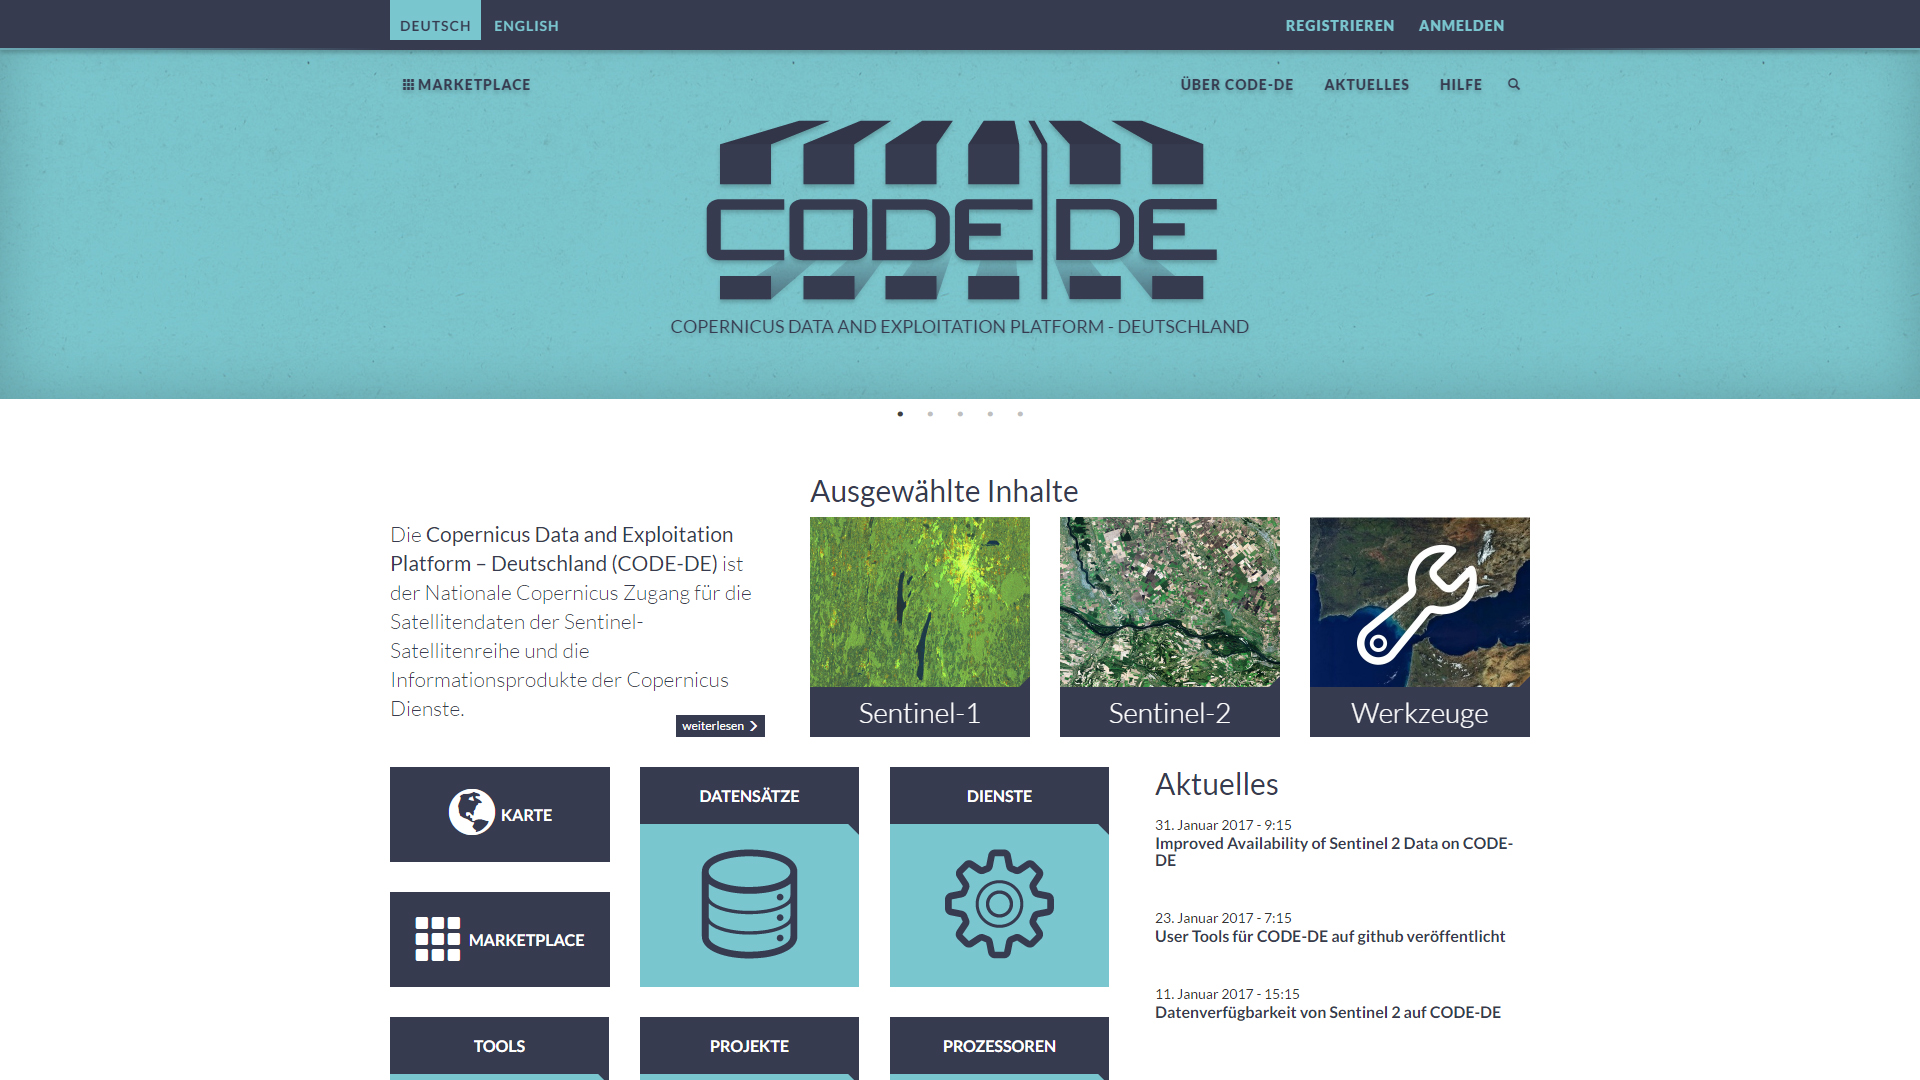
\includegraphics[width=1\textwidth]{images/cde_screen_0001_portal.jpg}\\
    
\href{https://code-de.org/}{code-de.org}
\end{frame}


\begin{frame}
  \frametitle{ TEP ESA }
 \includegraphics[width=1\textwidth]{images/esa_tep.jpg}\\
  
\href{https://tep.eo.esa.int/}{ESA Thematic Exploitation Platforms (TEPs)} 
 
\end{frame}

\begin{frame}
  \frametitle{REDD+ cloud computing tool}

\begin{tikzpicture} %[spy using overlays]
\node (pic1) [inner sep=0pt] {\includegraphics[width=0.3\textwidth,keepaspectratio=true]{./images/sepal_satpics}};

\node (pic2) [inner sep=0pt, anchor=west, yshift=1.5cm, xshift=-.5cm, ] at (pic1.east) {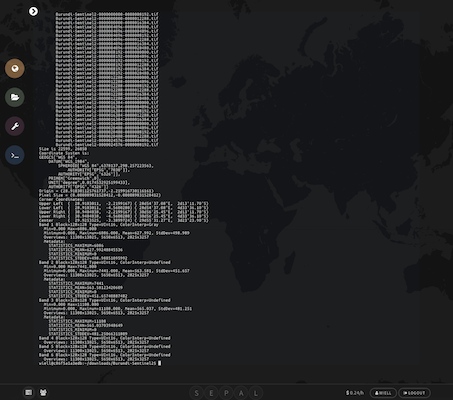
\includegraphics[width=0.3\textwidth]{images/sepal_metadata.png}};
\node (pic3) [inner sep=0pt, anchor=west, yshift=1.5cm, xshift=-.5cm, ] at (pic2.east) {\includegraphics[width=0.3\textwidth]{images/sepal_outout.png}};

\node (link1) [inner sep=0pt, anchor=west, yshift=-2cm, xshift=-.5cm, ] at (pic3.south) {Link: \href{https://sepal.io/}{  sepal.io  } };

\end{tikzpicture}

% node[fill=red!20, ] {3rd node};

\end{frame}

\begin{frame}
  \frametitle{ JICA-JAXA }
 \begin{center}
 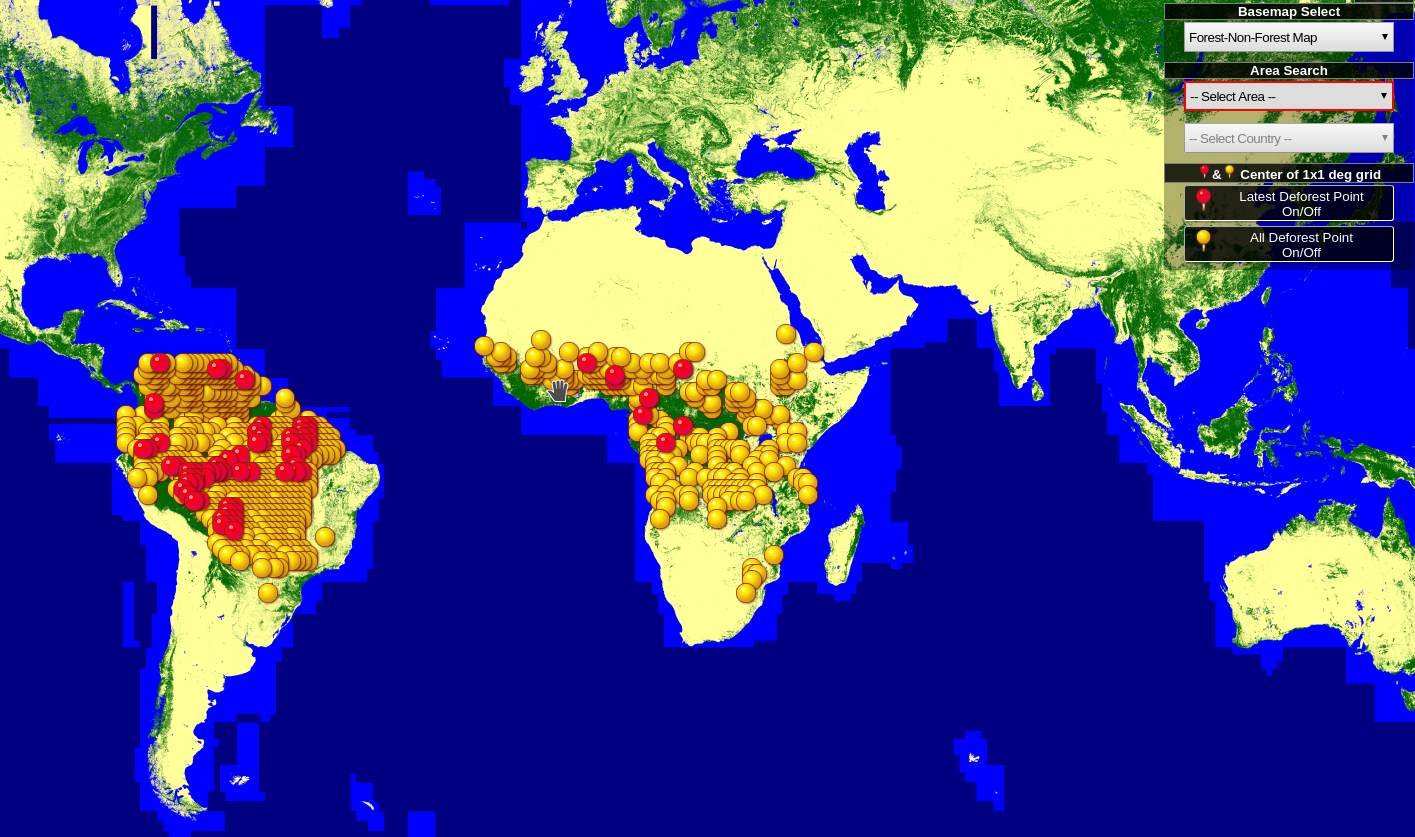
\includegraphics[width=0.9\textwidth,keepaspectratio=true]{./images/jjfast.png}
 % jjfast.png: 0x0 pixel, 300dpi, 0.00x0.00 cm, bb=
\end{center} 

\href{http://www.eorc.jaxa.jp/jjfast/}{JICA-JAXA Forest Early Warning System in the Tropics }
\end{frame}

\begin{frame}
  \frametitle{Trends.earth QGIS plugin (UNCCD LDN --> SDG 13.5.1)} 

\begin{tikzpicture} %[spy using overlays]
\node (pic1) [inner sep=-20pt] {\includegraphics[height=0.25\textheight]{images/trendsearth-0.png}};

\node (pic2) [inner sep=0pt, anchor=west, yshift=1.5cm, xshift=-.5cm, ] at (pic1.east) {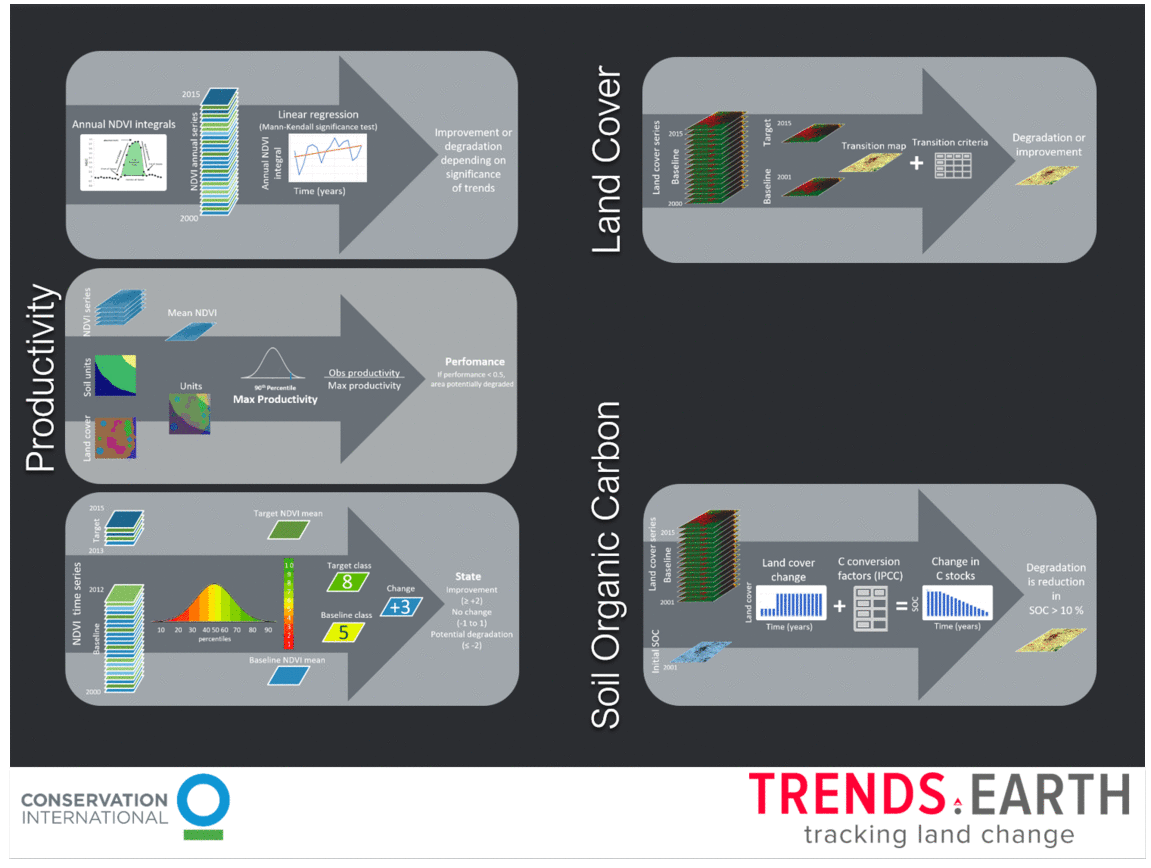
\includegraphics[width=0.3\textwidth]{images/trendsearth-1.png}};


\node (pic3) [inner sep=0pt, anchor=west, yshift=1.5cm, xshift=-1cm, ] at (pic2.east) {\includegraphics[width=0.3\textwidth]{images/trendsearth-2.png}};


\node (pic4) [inner sep=0pt, anchor=north, yshift=-.8cm, xshift=1.5cm, ] at (pic3.south) {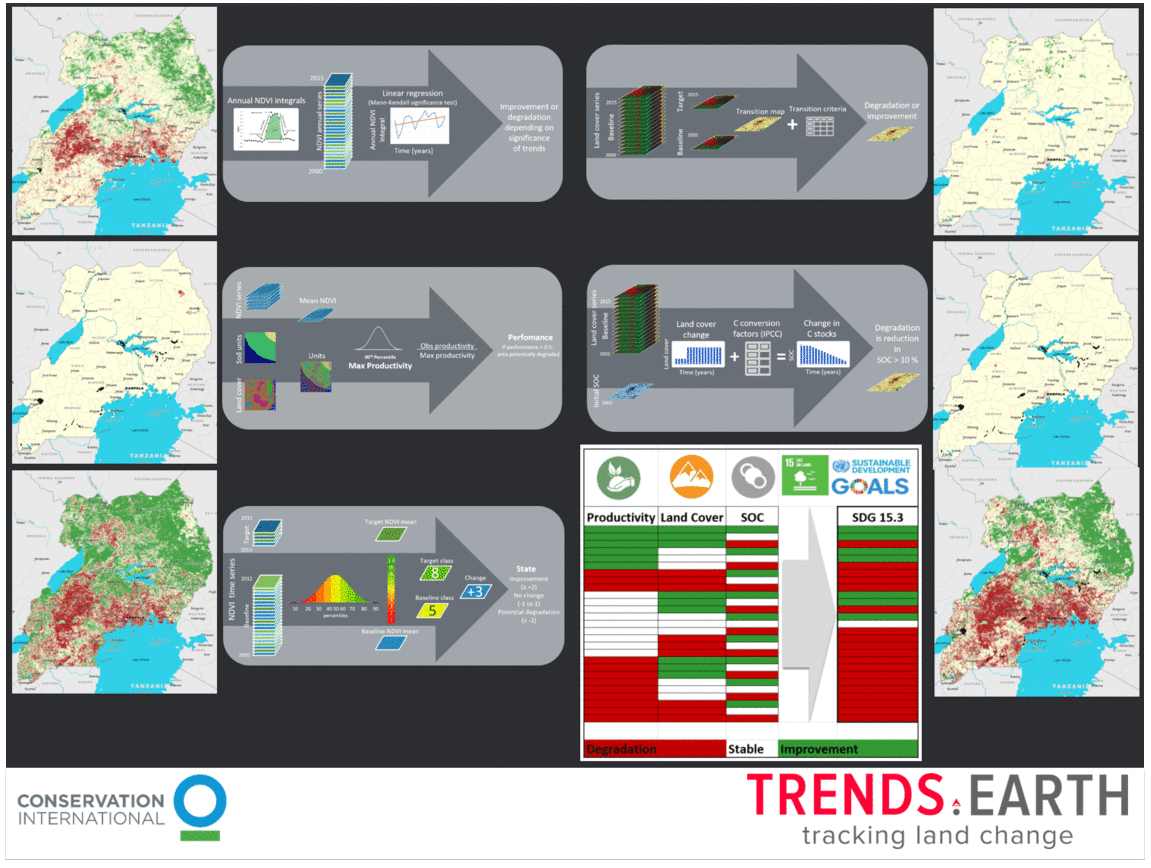
\includegraphics[width=0.3\textwidth]{images/trendsearth-3.png}};


\node (pic5) [inner sep=0pt, anchor=west, yshift=1.5cm, xshift=-1.2cm, ] at (pic4.east) {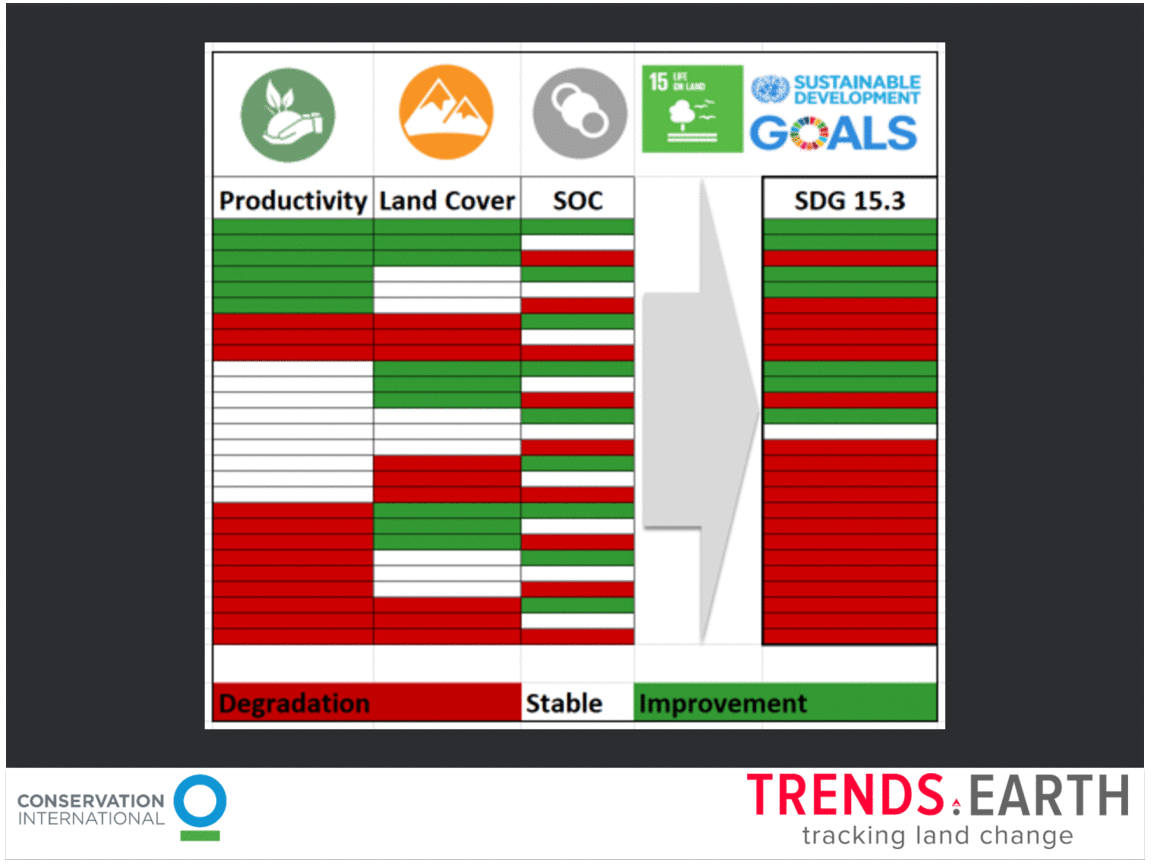
\includegraphics[width=0.3\textwidth]{images/trendsearth-4.png}};


\node (pic6) [inner sep=0pt, anchor=west, yshift=1.7cm, xshift=-1.4cm, ] at (pic5.east) {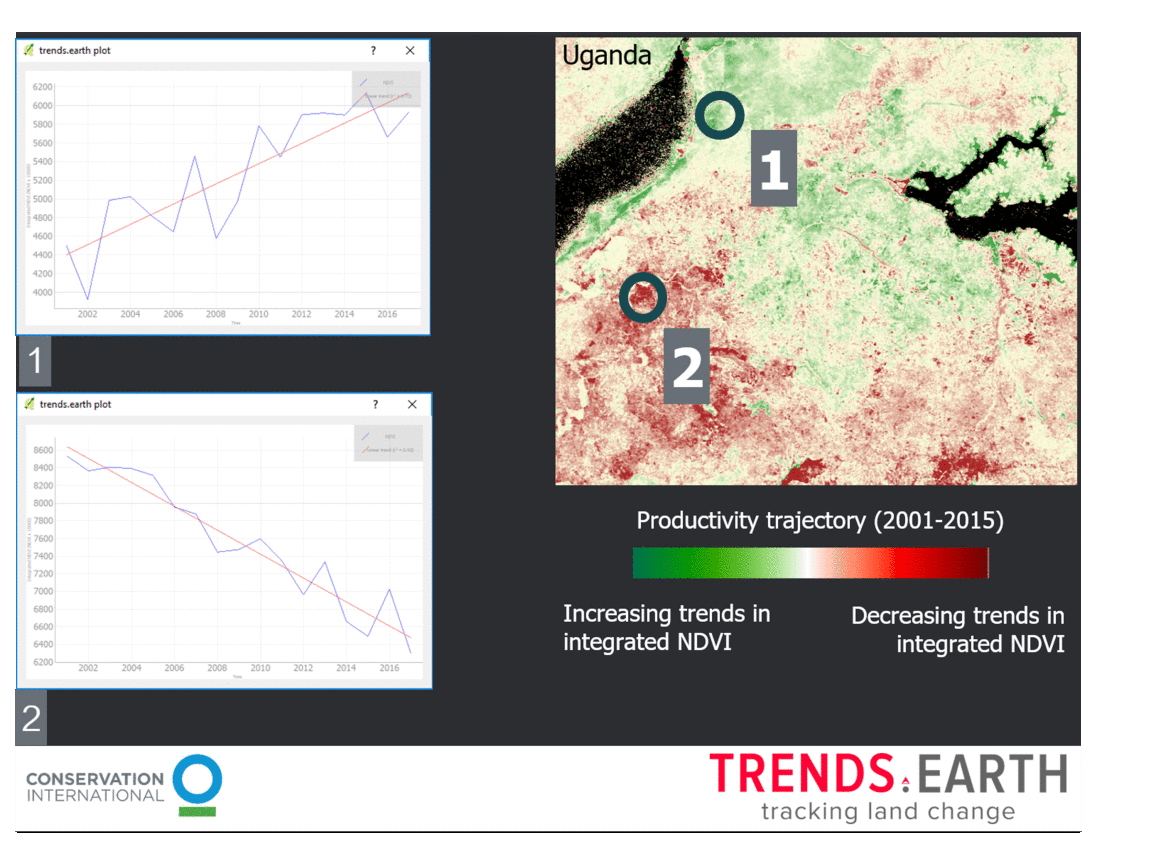
\includegraphics[width=0.3\textwidth]{images/trendsearth-5.png}};
   
   
\end{tikzpicture}

\centering
\href{ http://trends.earth/docs/en/}{link to Documentation Trends.Earth}\\
\href{http://trends.earth/docs/en/documentation/info.html}{link to  Tutorial Trends.Earth}

\end{frame}

\begin{frame}
  \frametitle{ODC}
\vspace{-1.5cm}
\begin{figure}[ht]
	\centering
	\includegraphics[width=0.8\textwidth, page=3]{./images/Sims_SamoaODC_23May2018.pdf}
   % \caption{(Regional Data Cubes \tiny{(Thanks to Neil Sims CEOS)}}
\end{figure}
\href{https://www.opendatacube.org/}{opendatacube}\\
\href{https://www.earthobservations.org/documents/meetings/201805_rapp_sdg_odc/201805_odc_announcement.pdf}{Link: African Regional Data Cube Announcement}\\
\vspace{0.5cm}
Video Links:\\ 
\href{https://www.youtube.com/watch?v=tEeT5VH7qVc}{Africa Regional Data Cube}\\
\href{https://www.youtube.com/watch?v=exIBPwtvbiI}
{How the Data Revolution is Shaping Africa's Future}

\end{frame}

% \begin{frame}
%   \frametitle{ Rangeland and pasture productivity }
%    http://map.geo-rapp.org/
% \end{frame}



\section[Technique]{Technical Aspects}
\AtBeginSection[]
{
  \begin{frame}<beamer>
    \frametitle{Technical Aspects \thesection}
    \tableofcontents[currentsection]
  \end{frame}
}

% \begin{frame}
% \frametitle{The Big Data problem}
% 
% \begin{center}
%  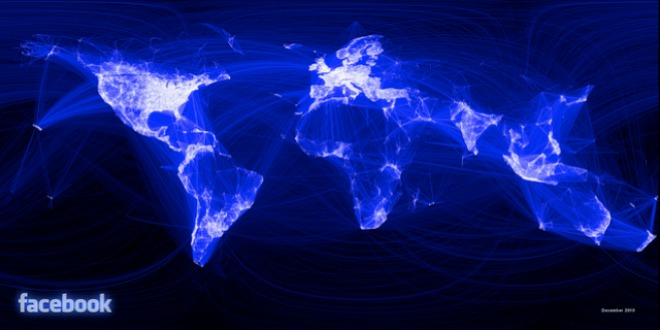
\includegraphics[width=\textwidth]{./images/internetconnection.png}
%  % wps_principe_fr.png: 0x0 pixel, 300dpi, 0.00x0.00 cm, bb=
% \end{center}
% \end{frame}


\begin{frame}

\frametitle{Open Data Cubes (OCD)}
\vspace{-1cm}
 \includegraphics[height=\textheight, page=1]{./images/Sims_SamoaODC_23May2018.pdf}
 % earth-on-aws-nextgeneration-open-data-platforms-25-1024.jpg: 0x0 pixel, 300dpi, 0.00x0.00 cm, bb=

\end{frame}

\begin{frame}

\frametitle{Network Common Data Format (netCDF) }

 \includegraphics[width=1.1\textwidth]{./images/netCDF_schema.png}
 % earth-on-aws-nextgeneration-open-data-platforms-25-1024.jpg: 0x0 pixel, 300dpi, 0.00x0.00 cm, bb=

\end{frame}



\begin{frame}

\frametitle{Web Processing Services}
\begin{center}
 \includegraphics[width=\textwidth]{./images/wps_principe_fr.png}
 % wps_principe_fr.png: 0x0 pixel, 300dpi, 0.00x0.00 cm, bb=
\end{center}

\end{frame}


\begin{frame}

\frametitle{OGC Standard}

\includegraphics[width=\textwidth]{./images/OGC_webservices.jpg}


\end{frame}

\begin{frame}

\frametitle{Birdhouse-PAVICS framework}

\begin{center}
 \vspace{-0.5cm}
 \includegraphics[width=1.1\textwidth]{./images/PAVICS_architecture.png}
 % wps_principe_fr.png: 0x0 pixel, 300dpi, 0.00x0.00 cm, bb=
\end{center}

\end{frame}




\begin{frame}{ Ingredients of the recipe for data for SDGs }

\begin{tikzpicture}[
    myarrow/.style={single arrow,single arrow head extend=.1cm,anchor=east,minimum height=1.8cm,minimum width=.8cm},
    myrectangle/.style={rectangle,rounded corners=2,draw=white,text=white,inner sep=.5cm,align=center}]

\node(a)[draw=myblue,circle,fill=yellow,text=white,inner sep=.2cm,outer sep=.2cm]{\href{http://www.data4sdgs.org/}{data4sdgs.org}};
\node(b)[draw=myred,fill=myred,myarrow]at(a.west){};
\node(c)[draw=mygreen,fill=mygreen,myarrow,rotate=-45]at(a.north west){};
\node(d)[draw=myviolet,fill=myviolet,myarrow,rotate=-90]at(a.north){};
\node(e)[draw=myturquoise,fill=myturquoise,myarrow,rotate=-135]at(a.north east){};
\node(f)[draw=myorange,fill=myorange,myarrow,rotate=-180]at(a.east){};
\node(g)[myrectangle,fill=myred,anchor=east]at(b.mid){Open Data Policy\\Copy Left License};
\node(g)[myrectangle,fill=mygreen,anchor=south east]at(c.mid){FOSS4G\\OGC};
\node(g)[myrectangle,fill=myviolet,anchor=south]at(d.mid){UNFCCC\\UNCCD\\SDG\\etc.};
\node(g)[myrectangle,fill=myturquoise,anchor=south west]at(e.mid){OPC\\WPS\\WMS\\etc...};
\node(g)[myrectangle,fill=myorange,anchor=west]at(f.mid){\href{https://scihub.copernicus.eu/}{COPERNICUS.hub}\\ \href{https://esgf-data.dkrz.de/projects/esgf-dkrz/}{ESGF-data}\\\href{https://www.gbif.org/}{GBIF.org}\\etc...};
%\node(a)[draw=myblue,circle,fill=myblue,text=white,inner sep=.2cm,outer sep=.2cm]{ Data based sustainable development };
% \node(b)[draw=myred,fill=myred,myarrow]at(a.west){};
% \node(c)[draw=mygreen,fill=mygreen,myarrow,rotate=-45]at(a.north west){};
% \node(d)[draw=myviolet,fill=myviolet,myarrow,rotate=-90]at(a.north){};
% \node(e)[draw=myturquoise,fill=myturquoise,myarrow,rotate=-135]at(a.north east){};
% \node(f)[draw=myorange,fill=myorange,myarrow,rotate=-180]at(a.east){};
% \node(g)[myrectangle,fill=myred,anchor=east]at(b.mid){Open Data\\policy};
% \node(g)[myrectangle,fill=mygreen,anchor=south east]at(c.mid){OGC\\interoperability};
% \node(g)[myrectangle,fill=myviolet,anchor=south]at(d.mid){UNFCCC\\UNCCD\\SDG};
% \node(g)[myrectangle,fill=myturquoise,anchor=south west]at(e.mid){datacubes\\WPS};
% \node(g)[myrectangle,fill=myorange,anchor=west]at(f.mid){FOSS};
\end{tikzpicture}
\hspace{2cm}


\end{frame}

\section{DEMO Session / Tutorials}

\begin{frame}{ DEMO }

\href{https://pavics.ouranos.ca/}{Platform Visualisation Climate Services}\\
\vspace{1cm}
\href{http://13.59.149.225/}{African Regional Data Cubes}\\ 
\vspace{1cm}

\href{http://birdhouse-workshop.readthedocs.io/en/latest/}{WPS 
Workshop}\\
\vspace{1cm}
\href{https://sepal.io/}{REDD+ sepal.io/}
\end{frame}

\end{document}

